% This is samplepaper.tex, a sample chapter demonstrating the
% LLNCS macro package for Springer Computer Science proceedings;
% Version 2.20 of 2017/10/04
%
\documentclass[runningheads]{llncs}
%
\usepackage{graphicx}
\usepackage{titling}
\usepackage{amssymb}
% Used for displaying a sample figure. If possible, figure files should
% be included in EPS format.
%
% If you use the hyperref package, please uncomment the following line
% to display URLs in blue roman font according to Springer's eBook style:
% \renewcommand\UrlFont{\color{blue}\rmfamily}

%\pretitle{%
%  \begin{center}
%  \LARGE
%  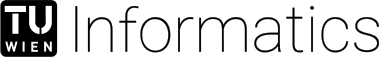
\includegraphics[width=.3\textwidth]{logo.png}\\
%}
%\posttitle{\end{center}}

\usepackage{etoolbox}
\makeatletter
\providecommand{\subtitle}[1]{% add subtitle to \maketitle
  \apptocmd{\@title}{\par {\large #1 \par}}{}{}
}
\makeatother


\begin{document}
%
\title{A graph visualization for the Hrafnkel dataset, \\or why you should never ride \\another man's horse}
\subtitle{asdasdasdasd}
%
\titlerunning{Abbreviated paper title}
% If the paper title is too long for the running head, you can set
% an abbreviated paper title here
%
\author{Tamara Drucks \and 
Moritz Leidinger \and 
Giulio Pace}
%
\authorrunning{Drucks et al.}
% First names are abbreviated in the running head.
% If there are more than two authors, 'et al.' is used.
%
\institute{TU Wien, Vienna, Austria} %\\
%\email{\{e11111111,e22222222,e11835706\}@student.tuwien.ac.at}
%
%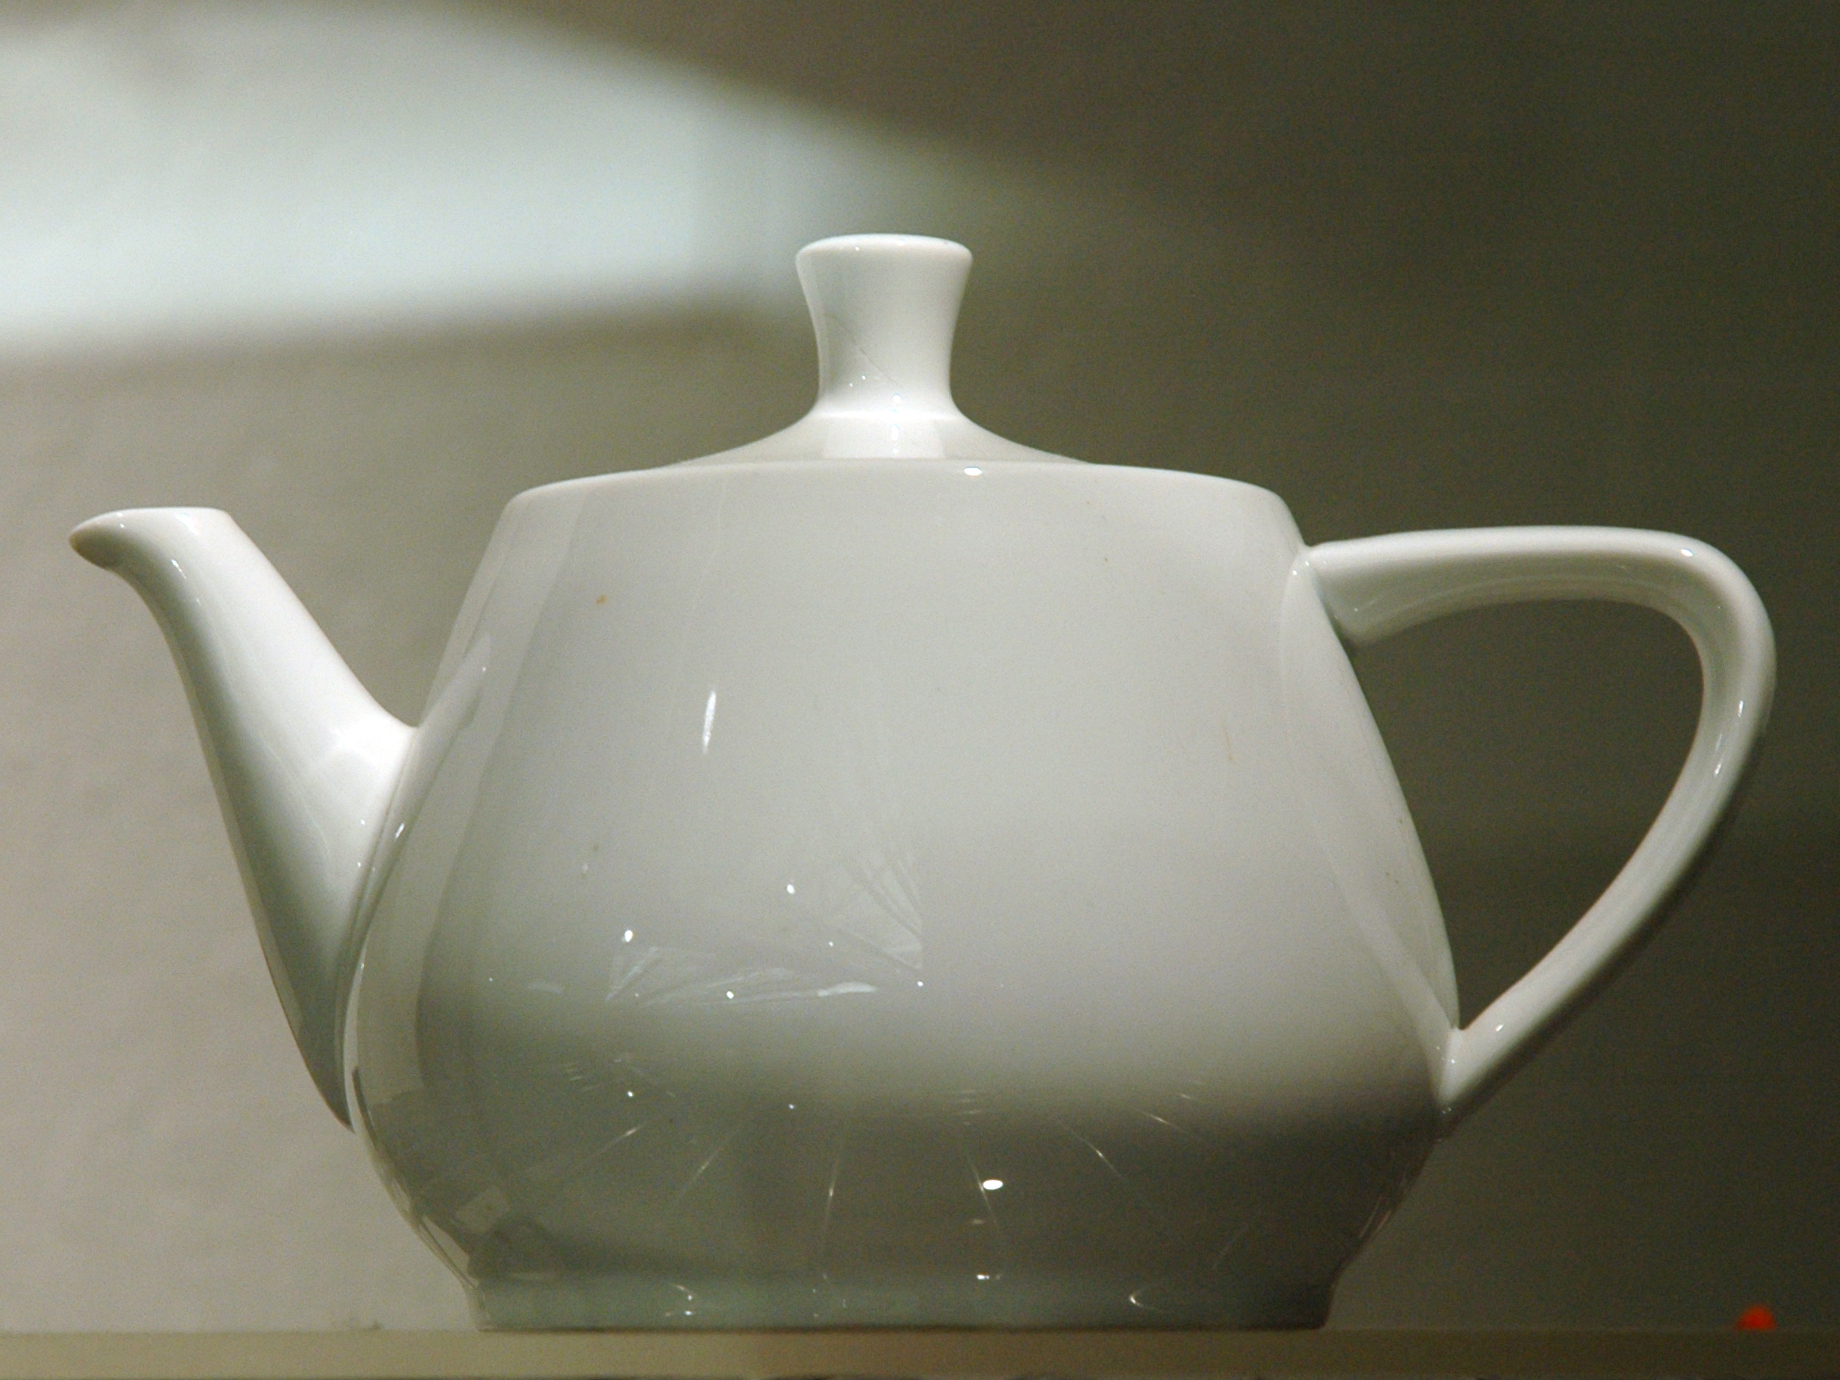
\includegraphics[width=.4\textwidth]{Original_Utah_Teapot.jpg}
\date{September 2020}
\maketitle              % typeset the header of the contribution
\vspace{-35pt}
\begin{figure}
	\centering
	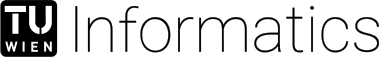
\includegraphics[width=.3\textwidth]{logo.png}
\end{figure}
\vspace{-25pt}
\section{Introduction}

We are Tamara Drucks, Moritz Leidinger and Giulio Pace from TU Wien and we present here our submission for the graph drawing creative competition for the Hrafnkel dataset.


\section{Stylistic choices}

To represent the graph in a more readable way we made some changes to the dataset:
\begin{itemize}
	\item In our representation, every character is a line (character line) that passes through the nodes that represent actions (action nodes), in a metro map fashion;
	\item For each character, except one-time occurrences, we added an origin and an end node: therefore each character is a collection of edges that connect multiple action nodes forming a path that starts at the origin node and ends at the end node. 
\end{itemize}
Characters are grouped and colored with respect to the families they belong to: 
\begin{itemize}
	\item Every family has a general color that helps to distinguish what group they come from;
	\item Every character has a specific shade of their family color assigned to her/him;
	\item Hrafnkel's family is blue because it was the color that was worn when killing people in the Icelandic tradition; 
	\item The divine characters are golden.
	\item Sam's family is red, as most blood is spilled there.
	\item The family of Thorgeir and Thorkel is green, as the latter was described to have worn green in the saga. 
\end{itemize}
This way the more common characters are the primary colors to improve the readability of the graph. \\
The graph is superimposed onto a map of Iceland to give a geographical localization to the events. We also wanted to give the graph the feeling of an old map. The family trees are roughly located in the area of Iceland they reside in. This is further underlined by a shading of the areas with the respective family color. \\
The character lines are organized in a spiral that represents the cyclic structure of the story.
%>>>REMOVE?? It is also visually pleasing and it tends to fit the places where the actions take place in the story.<<< 
The action nodes are organized in the order they appear in, in the story (with the exception of „hostility lethal“ towards the King of Greeks, which we could not find in any translation of the saga). We also separated the actual actions from the family actions that describe the relationships between the characters, which are evident in the family trees. The ultimate goal is to display the story as a timeline that gives a chronological direction to the actions as well as a geographical one. The latter was obviously not always possible and is quite generic, but we feel the graph succeeds in conveying this idea. \\

\section{How to read the graph}

The spiral starts from the north-east and unfolds through the map of Iceland to end close to the center of the island. Every action is represented by an icon in a circle. The icons are made by Freepik, photo3idea\_studio, Pixel Perfect, Becris, itim2101, Smashicons from the website www.flaticon.com. The color of the circular outline around the icon represents the person performing the action to the other character that is connected to the node. More information about how to read the action nodes and the meaning of the icons can be found in the legend on the bottom left corner of the poster. The line thicknesses represent the importance of the character measured in the number of actions they take part in. On the same note, characters that perform only one action do not have their own character line but appear only as a small line branching from the action they perform. One section of the graph which is devoted to a series of characters that were children of one another and was used to give a time reference to the readers of the saga. In this case we decided to use the text itself in the south east corner instead of creating a family tree for them. In our opinion this is a very nice start for the story and reporting it helps to give a general feeling of the story to the reader. \\
Finally, some characters in the dataset never perform any actions; it was a conscious design decision to exlude them from our representation, as they do not provide any additional information.




%The actual contest contribution should be inserted in a PDF merge tool as the second page. (Not via the \LaTeX\ includegraphics command as that would create an ugly white margin around it.)


%
% ---- Bibliography ----
%
% BibTeX users should specify bibliography style 'splncs04'.
% References will then be sorted and formatted in the correct style.
%
% \bibliographystyle{abbrv}
% \bibliography{references}
%
%\begin{thebibliography}{8}
%
%\end{thebibliography}
\end{document}
